% Created 2017-03-20 Mon 09:26
% Intended LaTeX compiler: pdflatex
\documentclass[bigger]{beamer}
\usepackage[utf8]{inputenc}
\usepackage[T1]{fontenc}
\usepackage{fixltx2e}
\usepackage{graphicx}
\usepackage{longtable}
\usepackage{float}
\usepackage{wrapfig}
\usepackage{rotating}
\usepackage[normalem]{ulem}
\usepackage{amsmath}
\usepackage{textcomp}
\usepackage{marvosym}
\usepackage{wasysym}
\usepackage{amssymb}
\usepackage{hyperref}
\tolerance=1000
\usepackage{minted}
\usepackage{mycmds}
\usepackage{pgfplots}
\usepackage[german, germanb]{babel}
\uselanguage{german}
\usepackage{url}
\usepackage{pgfplots}
\usetikzlibrary{pgfplots.groupplots}
\pdfmapfile{+sansmathaccent.map}
\mode<beamer>{\usetheme{Berkeley}}
\usetheme{default}
\author{Stephan Messlinger, Valentin Ochs}
\date{\today}
\title{Blinkenlights Workshop}
\hypersetup{
 pdfauthor={Stephan Messlinger, Valentin Ochs},
 pdftitle={Blinkenlights Workshop},
 pdfkeywords={},
 pdfsubject={},
 pdfcreator={Emacs 24.5.1 (Org mode 9.0.5)}, 
 pdflang={Germanb}}
\begin{document}

\maketitle

\section{Digital Out}
\label{sec:orgf1734bc}
\begin{frame}[fragile,label={sec:orgdeaa9ea}]{Startpunkt digitaler Output}
 Blink Beispiel: File \(\rightarrow\) Examples \(\rightarrow\) Basics \(\rightarrow\) Blink

\begin{minted}[]{c}
void setup() {
  pinmode(13, output);
}

void loop() {
  digitalwrite(13, high);
  delay(1000);
  digitalwrite(13, low);
  delay(1000);
}
\end{minted}
\end{frame}

\begin{frame}[fragile,label={sec:orgbdd5188}]{setup}
 \texttt{pinmode(pin, modus)} wählt für den Pin mit Nummer \texttt{pin} eine von drei
Betriebsarten:

\begin{itemize}
\item \texttt{OUTPUT}: wird für Ausgabe verwendet, z.B. um LEDs zu schalten oder
mit anderen Microcontrollern zu sprechen.
\item \texttt{INPUT}: die Spannung am Pin kann gelesen werden.
\item \texttt{INPUT\_PULLUP}: wie \texttt{INPUT}, aber der Pin wird intern auf die
Versorgunsspannung gezogen.
\end{itemize}
\end{frame}

\begin{frame}[fragile,label={sec:org63febe0}]{digitalWrite und Delay}
 \texttt{digitalWrite(pin, zustand)} setzt bei einem auf \texttt{OUTPUT} gestellten Pin
die Ausgangsspannung:

\begin{itemize}
\item 0 Volt für \texttt{LOW}
\item 5 Volt für \texttt{HIGH} (oder was auch immer die aktuelle
Versorgungsspannung ist)
\end{itemize}

\texttt{delay(ms)} tut \texttt{ms} Millisekunden lang nichts.
\end{frame}

\begin{frame}[fragile,label={sec:org70c608f}]{Andere Blink Muster}
 Zwei Sekunden lang an, eine halbe aus.

\pause

\begin{minted}[]{c}
void setup() {
  pinmode(13, output);
}

void loop() {
  digitalwrite(13, high);
  delay(2000);
  digitalwrite(13, low);
  delay(500);
}
\end{minted}
\end{frame}

\begin{frame}[label={sec:org11652d4}]{Schnelleres Blinken}
Was passiert, wenn man die Zeiten ganz niedrig setzt?
\pause

\(\rightarrow\) Man sieht kein Blinken mehr
\pause

Was passiert, wenn die Zeitverhältnisse geändert werden?
\pause

\(\rightarrow\) Dimmen
\end{frame}

\section{Analog Out}
\label{sec:orgef08f9b}
\begin{frame}[fragile,label={sec:org26bb56f}]{analogWrite}
 \texttt{analogWrite(pin, wert)} schaltet den Pin automatisch an und aus, mit
variablen An-/Aus-Zeiten 

\(\rightarrow\) Pulsweitenmodulation

\begin{itemize}
\item Frequenz: Etwa 490 Hz
\item Wertebereich: 0 bis 255
\item Nur auf Pins 3, 5, 6, 9, 10, und 11.
\item Die PWM Pins sind auf dem Arduino mit \textasciitilde{} markiert.
\end{itemize}
\end{frame}

\begin{frame}[label={sec:orgd0a2c72}]{PWM Funktionsweise: Zähler + Vergleich}
\begin{tikzpicture}
\begin{axis}[xlabel=Zeit / s, ylabel=Zähler, ymin=-0.02*256, ymax=1.02*256]
\addplot[blue, domain=0:0.001, samples=512] { floor(mod(x*490*2*pi*256, 256)) };
\addplot[red, domain=0:0.001, samples=2] { 128 };
\end{axis}
\end{tikzpicture}
\end{frame}

\begin{frame}[label={sec:orgd30fb8a}]{PWM, Schwellwert 128}
\begin{tikzpicture}
\begin{axis}[xlabel=Zeit / s, ylabel=Spannung / V, ymin=-0.1, ymax=5.1]
\addplot[blue, domain=0:0.001, samples=500] { 5*ceil(0.5-mod(x*490*2*pi, 1)) };
\addplot[red, domain=0:0.001, samples=2] { 2.5 };
\end{axis}
\end{tikzpicture}
\end{frame}

\begin{frame}[label={sec:org937eccc}]{PWM, Schwellwert 16}
\begin{tikzpicture}
\begin{axis}[xlabel=Zeit / s, ylabel=Spannung / V, ymin=-0.1, ymax=5.1]
\addplot[blue, domain=0:0.001, samples=500] { 5*ceil(0.0625-mod(x*490*2*pi, 1)) };
\addplot[red, domain=0:0.001, samples=2] { 16./256 };
\end{axis}
\end{tikzpicture}
\end{frame}

\begin{frame}[fragile,label={sec:orgf7ddd8b}]{Einfacher PWM Code}
 \begin{minted}[]{c}
int const led_pin = 11;
void setup() {
  pinMode(led_pin, OUTPUT);
}
void loop() {
  // Zeit seit Beginn des Programms
  unsigned long time = millis();
  // Berechne eine Sägezahn mit 0.1 Hz
  int value = 255 * time / 4000;
  // Verwende den Wert als Schwellwert
  analogWrite(led_pin, value);
}
\end{minted}
\end{frame}

\begin{frame}[fragile,label={sec:orgb4ec025}]{Datentypen (1)}
 \begin{itemize}
\item \texttt{unsigned long time} und \texttt{int value} definieren Variablen.
\item \texttt{unsigned long} und \texttt{int} sind die Typen, \texttt{time} und \texttt{value} die
Namen, bzw. Identifier.
\item Normal sind Typen vorzeichenbehaftet, durch \texttt{unsigned} haben sie
einen nicht-negativen Wertebereich
\item Kleinere Datentypen sind schneller
\end{itemize}

\begin{center}
\begin{tabular}{lll}
Typ & Wertebereich & \texttt{unsigned} Wertebereich\\
\texttt{char} & \(-2^7\)  bis \(2^7-1\) & 0 bis \(2^8-1\)\\
\texttt{int} & \(-2^{15}\) bis \(2^{15}-1\) & 0 bis \(2^{16}-1\)\\
\texttt{long} & \(-2^{31}\) bis \(2^{31}-1\) & 0 bis \(2^{32}-1\)\\
\end{tabular}
\end{center}
\end{frame}

\begin{frame}[fragile,label={sec:org4f8bf6f}]{Datentypen (2)}
 \begin{itemize}
\item \texttt{float} für Gleitkommazahlen (sehr langsam!)
\item \texttt{double} für genauere Gleitkommazahlen (unglaublich langsam)
\item \texttt{const} Suffix (z.B. \texttt{int const}) für Werte, die sich nach ihrer
Definition nicht ändern. Vorteile:
\begin{itemize}
\item Etwas lesbarer
\item Kann zu schnelleren Programmen führen
\end{itemize}
\item Zu gro\ss{}e (oder kleine) Werte führen zu Überlauf:
\begin{itemize}
\item Bei \texttt{char}: 127+1 \(\rightarrow\) -128
\item Bei \texttt{unsigned char}: 0 - 1 \(\rightarrow\) 255
\end{itemize}
\end{itemize}
\end{frame}

\begin{frame}[label={sec:orge615a93}]{PWM Frequenz}
490 Hz sind bei schnellen Bewegungen sichtbar.

Bestimmung der Frequenz: Taktfrequenz / Vorteiler / Zählergrö\ss{}e

\begin{itemize}
\item Taktfrequenz: 16 MHz
\item Zählergrö\ss{}e:
\begin{itemize}
\item 256 für Pins 5 und 6
\item 510 für 3, 9, 10, 11
\end{itemize}
\end{itemize}
\end{frame}

\begin{frame}[fragile,label={sec:orge9067be}]{PWM Vorteiler: Timer 0, Pins 5 und 6}
 \begin{center}
\begin{tabular}{rrr}
Einstellung & Teiler & Frequenz\\
\hline
0x01 & 1 & 62500\\
0x02 & 8 & 7813\\
0x03 & 64 & 977\\
0x04 & 256 & 244\\
0x05 & 1024 & 61\\
\end{tabular}
\end{center}

Einstellen durch
\begin{minted}[]{c}
TCCR0B = (TCCR0B & 0b11111000) | Einstellung
\end{minted}
\end{frame}

\begin{frame}[fragile,label={sec:org480b062}]{PWM Vorteiler: Timer 1, Pins 9 und 10}
 \begin{center}
\begin{tabular}{rrr}
Einstellung & Teiler & Frequenz\\
\hline
0x01 & 1 & 31373\\
0x02 & 8 & 3921\\
0x03 & 64 & 490\\
0x04 & 256 & 123\\
0x05 & 1024 & 31\\
\end{tabular}
\end{center}

Einstellen durch
\begin{minted}[]{c}
TCCR1B = (TCCR0B & 0b11111000) | Einstellung
\end{minted}
\end{frame}

\begin{frame}[fragile,label={sec:orgde81372}]{PWM Vorteiler: Timer 2, Pins 11 und 3}
 \begin{center}
\begin{tabular}{rrr}
Einstellung & Teiler & Frequenz\\
\hline
0x01 & 1 & 31373\\
0x02 & 8 & 3921\\
0x03 & 32 & 980\\
0x04 & 64 & 490\\
0x05 & 128 & 245\\
0x06 & 256 & 123\\
0x07 & 1024 & 31\\
\end{tabular}
\end{center}

Einstellen durch
\begin{minted}[]{c}
TCCR2B = (TCCR2B & 0b11111000) | Einstellung
\end{minted}
\end{frame}

\begin{frame}[fragile,label={sec:org0fab25d}]{Vorsicht}
 Frequenzänderung beeinflusst nicht nur LEDs, sondern alles, was an dem
Timer hängt! Servos, Tonerzeugung, etc.

Besonders wichtig: Timer 0 für \texttt{millis()} und
\texttt{delay()}. Standardvorteiler: 64. Bei Änderungen Zeiten entsprechend
anpassen (Vervierfachen bei 256\ldots{})
\end{frame}

\section{Digital In}
\label{sec:org37f639d}
\begin{frame}[label={sec:org83d0818}]{Startpunkt digitaler Input}
Button Beispiel: File \(\rightarrow\) Examples \(\rightarrow\) Digital
\(\rightarrow\) Button

Geht nicht nur mit einfachen Schaltern und Tastern, sondern auch
z.B. einer Lichtschranke oder Reed-Schaltern.
\end{frame}

\begin{frame}[fragile,label={sec:org337a64a}]{digitalRead}
 \texttt{digitalRead(pin)}: 
\begin{itemize}
\item \texttt{HIGH} falls Spannung an \texttt{pin} etwa 2.6 V oder höher
\item \texttt{LOW} falls Spannung an \texttt{pin} 2.1 V oder tiefer
\item Nur bei 5 V Versorgungsspannung, sonst andere Werte
\end{itemize}
\end{frame}

\begin{frame}[label={sec:orgd4dd171}]{Schaltplanvarianten}
\begin{center}
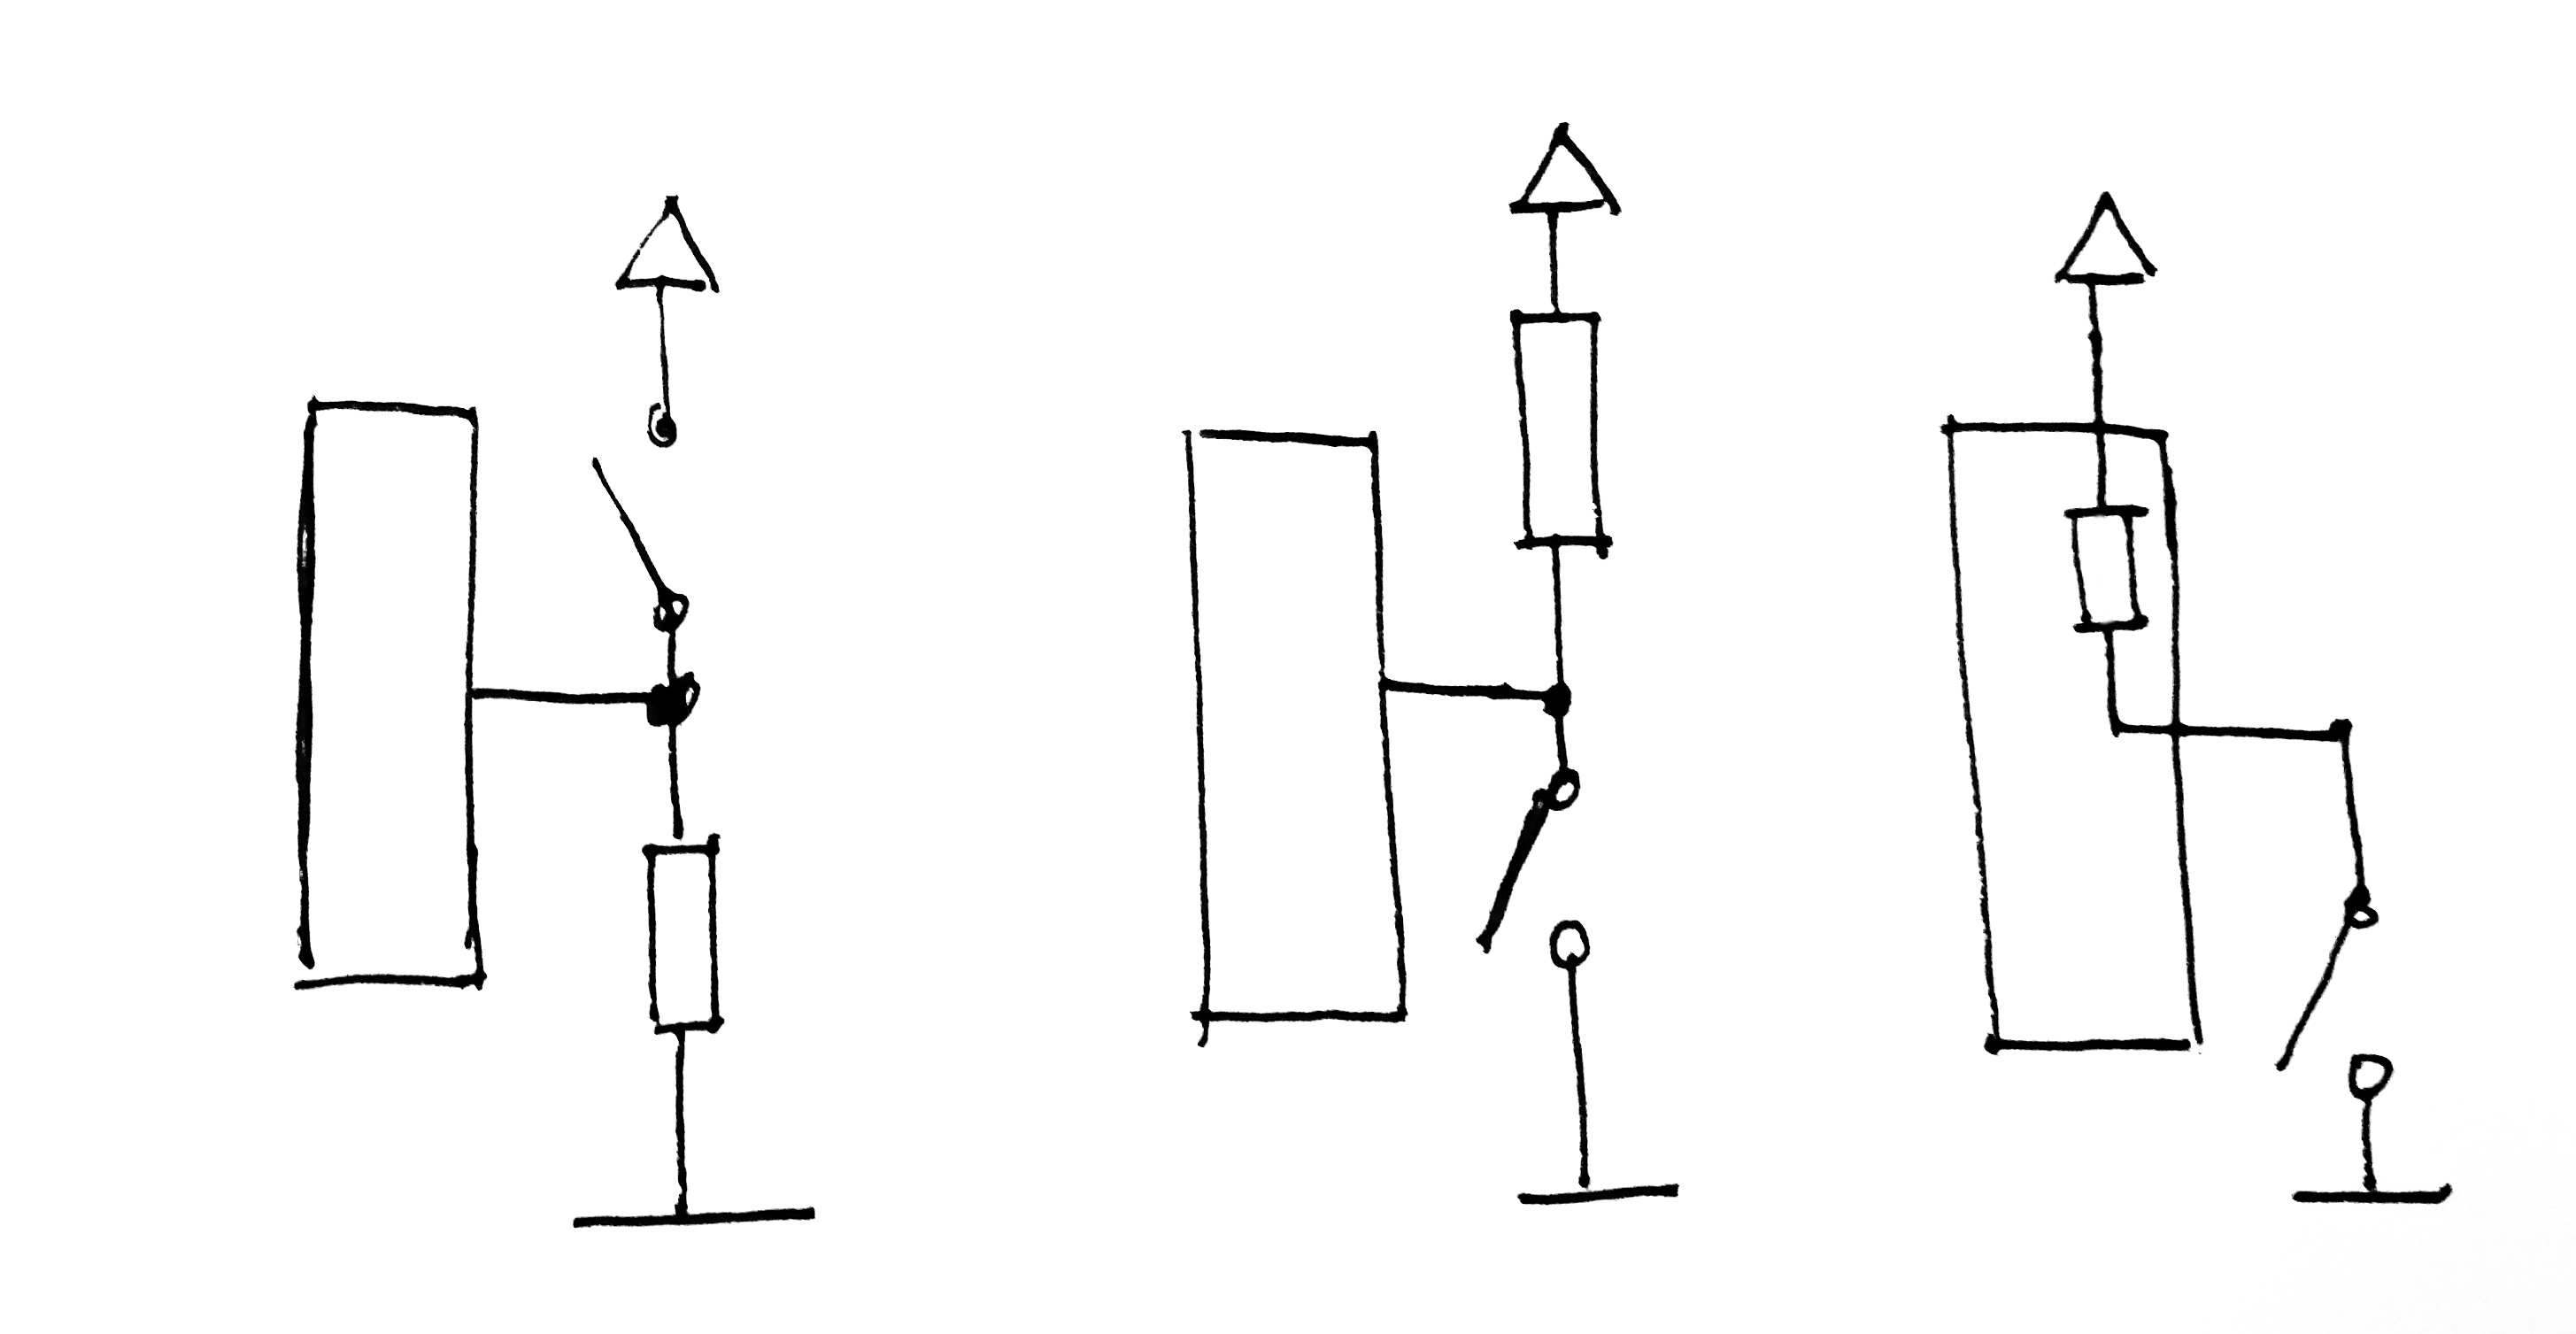
\includegraphics[width=.9\linewidth]{./img/pullup.jpg}
\end{center}
\end{frame}

\begin{frame}[fragile,label={sec:org1bfb978}]{Unterbrechbare Abläufe starten (1)}
 \begin{minted}[]{c}
unsigned long button_time = 0;
bool running = false;
void setup() {}
void loop() {
  if(digitalRead(button_pin) == HIGH) {
    running = true;
    button_time = millis();
  }
  if(running) {
    running = do_stuff(millis() - start_time);
  }
}
\end{minted}
\end{frame}

\begin{frame}[fragile,label={sec:org12d6a6d}]{Unterbrechbare Abläufe starten (2)}
 \begin{minted}[]{c}
bool do_stuff(unsigned long time_point)
  if(time_point < 100) {
    digitalWrite(led_pin, HIGH);
  } else if(time_point < 200) {
    digitalWrite(led_pin, LOW);
  } else if(time_point < 1000) {
    digitalWrite(led_pin, HIGH);
  } else {
    return false;
  }
  return true;
}
\end{minted}
\end{frame}

\begin{frame}[label={sec:org720126d}]{Prellen}
\begin{center}
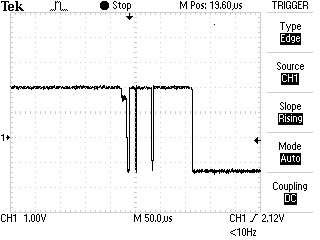
\includegraphics[width=.9\linewidth]{./img/bounce.png}
\end{center}
\end{frame}

\begin{frame}[label={sec:org4e7fb6f}]{Entprellen}
Auch: Debouncing

\begin{itemize}
\item Hardware Lösung: Tiefpassfilter mit Kondensator
\item Software Lösung: Mehrmals Wert auslesen und warten, bis er sich
nicht mehr ändert
\item Hier ohne weitere Vertiefung, aber ihr wisst jetzt, wonach man
suchen muss :)
\end{itemize}
\end{frame}

\section{Analog In}
\label{sec:orgfd0dcc1}
\begin{frame}[label={sec:orga5bdaa2}]{Startpunkt analoger Input}
AnalogInput Beispiel: File \(\rightarrow\) Examples \(\rightarrow\) Analog
\(\rightarrow\) AnalogInput
\end{frame}

\begin{frame}[fragile,label={sec:org99a21d8}]{analogRead}
 \texttt{analogRead(pin)}: 0-1023 für 0-5 Volt an Pin \texttt{pin}.
\end{frame}

\begin{frame}[fragile,label={sec:org2ad0f16}]{Kombination mit analogWrite}
 \begin{minted}[]{c}
void setup() {
    pinMode(3, OUTPUT);
}
void loop() {
    // Teile durch 4, um den
    // Wertebereich anzupassen
    int value = analogRead(A0) / 4;
    analogWrite(3, value);
}
\end{minted}
\end{frame}

\begin{frame}[fragile,label={sec:org3804105}]{An den PC senden}
 \begin{minted}[]{c}
void setup() {
  Serial.begin(115200);
}
void loop() {
  Serial.print("Aktueller Wert: ");
  Serial.println(analogRead(A0));
}
\end{minted}

Auch zur Fehlersuche nützlich!

Die Arduino IDE hat einen Plotter, mit dem man den zeitlichen Verlauf
von Zahlen beobachten kann.
\end{frame}

\begin{frame}[label={sec:org9654374}]{Spannungsbereich}
Maximale Spannung: Versorgungsspannung
\pause

Darüber: Spannungsteiler
\end{frame}

\section{Bunte Dinge}
\label{sec:org33c00a8}
\begin{frame}[label={sec:orgf251643}]{Macht Stephan}
\end{frame}

\section{Mehrere LEDs}
\label{sec:org4807f79}
\begin{frame}[label={sec:org02c4d24}]{Diskret}
Vorteile:
\begin{itemize}
\item Einfach
\item PWM (bei bis zu 6) möglich
\end{itemize}

Nachteile:
\begin{itemize}
\item 1 Pin pro LED
\item Ab 7 LEDs kein PWM mehr (oder nur in Gruppen)
\item 1 RGB LED braucht 3 Pins
\end{itemize}
\end{frame}

\begin{frame}[label={sec:org3c83774}]{Matrix}
Vorteile:
\begin{itemize}
\item Kann je nach Methode mit \(n\) Pins bis zu \(n^2-n\) LEDs ansteuern
\end{itemize}

Nachteile:
\begin{itemize}
\item Kompliziert
\item Niedrige Wiederholrate
\item Reduzierte Helligkeit
\item Bei grö\ss{}eren Spitzenströmen werden externe Treiber benötigt
\item Kein (hardware-beschleunigtes) Dimmen
\end{itemize}
\end{frame}

\begin{frame}[label={sec:orgd99889e}]{Schieberegister}
\begin{itemize}
\item Englisch: Shift register
\item Mehrere Ausgänge, z.B. 8
\item Digitale Steuerung, z.B. SPI oder I2C
\item Zu viele Werte \(\rightarrow\) alte Werte werden weitergeschoben
\end{itemize}

Vorteile:
\begin{itemize}
\item Einfach
\item Benötigt wenige (i.d.R. < 4) Pins
\item Leicht erweiterbar
\end{itemize}

Nachteile:
\begin{itemize}
\item Kein (hardware-beschleunigtes) Dimmen
\item Wiederholrate sinkt mit 1/n
\end{itemize}
\end{frame}

\section{LED Streifen}
\label{sec:orgbffc90a}
\begin{frame}[label={sec:org46736ad}]{WS2812, APA102\ldots{}}
\begin{itemize}
\item Mehrere LEDs auf Streifen
\item Ähnlich zu Schieberegistern
\item Eingebaute Logik zum Dimmen
\item Ansteuerung durch fertige Libraries
\end{itemize}
\end{frame}

\begin{frame}[label={sec:orgd246827}]{Libraries}
\begin{itemize}
\item Sketch \(\rightarrow\) Include Library \(\rightarrow\) Manage Libraries
\item Modularer Code, bei Arduino häufig zum Ansteuern von externer Hardware
\item Für WS2812: Adafruit NeoPixel
\item Für APA102: APA102
\end{itemize}
\end{frame}

\begin{frame}[fragile,label={sec:org7bd93cc}]{Beispielcode}
 \begin{minted}[]{c}
#include <Adafruit_NeoPixel.h>
Adafruit_NeoPixel strip(144, 13,
                        NEO_GRB + NEO_KHZ800);
int i = 0;
void setup() { strip.begin(); }
void loop() {
  strip.setPixelColor(i, 255, 0, 0);
  strip.show();
  delay(10);
  strip.setPixelColor(i, 0, 0, 0);
  i++;
  if(i == 144) i = 0;
}
\end{minted}
\end{frame}

\begin{frame}[fragile,label={sec:orgd55b74c}]{Arrays}
 \ldots{} speichern viele Werte gleichen Typs unter einem Namen. Das erste
Element hat Index 0.

Beispiel:
\begin{minted}[]{c}
int many_values[20];
for(int i = 0; i < 20; i++)
  many_values[i] = i;
Serial.print(many_values[0]+many_values[19]);
\end{minted}
\end{frame}

\begin{frame}[fragile,label={sec:orgf235a4d}]{Laufender Regenbogen}
 \setbeamerfont{smaller}{size=\scriptsize}
\usebeamerfont{smaller}
\begin{minted}[]{c}
#include <Adafruit_NeoPixel.h>
Adafruit_NeoPixel strip(144, 13, NEO_GRB + NEO_KHZ800);
uint32_t colors[144];
int i = 0;
void setup() {
  strip.begin();
  for(i = 0; i < 48; i++) {
    unsigned char v = i*255/48;
    colors[i]    = strip.Color(255-v, v, 0);
    colors[i+48] = strip.Color(0, 255-v, v);
    colors[i+96] = strip.Color(v, 0, 255-v);
  }
}
void loop() {
  for(int j = i; j < 144-i; j++)
    strip.setPixelColor(i+j,     colors[j]);
  for(int j = 144-i; j < 144; j++)
    strip.setPixelColor(i+j-144, colors[j]);
  strip.show();
  i++;
  if(i == 144) i = 0;
}
\end{minted}
\end{frame}

\section{Stromversorgung}
\label{sec:org149f4e9}
\begin{frame}[label={sec:orgf510b49}]{Macht Stephan}
\end{frame}

\section{Sensoren}
\label{sec:orgc8d8fb2}
\begin{frame}[label={sec:orge3c6606}]{Anschluss von Sensoren}
\begin{itemize}
\item Analog: Sensor giebt eine Spannung aus, die gemessen wird
\begin{itemize}
\item Unkompliziert, aber durch den Arduino eingeschränkte Genauigkeit,
Präzision, Geschwindigkeit, Anzahl von Sensoren
\end{itemize}
\item Digital: Sensor wird durch ein serielles Interface (häufig SPI oder
I2C) an den Arduino angeschlossen.
\begin{itemize}
\item Erlaubt manchmal auch Einstellungen (Messfrequenz, -bereich)
\item Etwas komplizierter zu programmieren
\item Viele Sensoren an wenigen Pins möglich
\end{itemize}
\end{itemize}
\end{frame}

\begin{frame}[label={sec:org0962667}]{Sensorbeispiele}
\begin{itemize}
\item Beschleunigung
\item Drehrate
\item Magnetfeld
\item Spannung
\item Luftfeuchtigkeit, Temperatur, Druck
\item Licht
\item Position (GPS)
\end{itemize}
\end{frame}

\begin{frame}[fragile,label={sec:orgf4fa527}]{Sensoren im Arduino}
 Spannung (analoger Input) und Temperatur (interne Temperatur, wird
über den Analog-Digital-Wandler gemessen).

\begin{minted}[]{c}
void setup() {
  Serial.begin(115200);
  // Temperaturmessung einrichten:
  ADMUX = (_BV(REFS1) | _BV(REFS0) | _BV(MUX3));
  ADCSRA |= _BV(ADEN);
}
void loop() {
  ADCSRA |= _BV(ADSC); // Messung starten
  while(ADCSRA & _BV(ADSC)) { } // Warte
  Serial.println(ADCW); // Wert ausgeben
}
\end{minted}
\end{frame}
\section{Basteln}
\label{sec:org25a4807}
\begin{frame}[label={sec:orgfdbd452}]{Basteln}
Vorschläge?

Mehr als ausreichend vorhanden:
\begin{itemize}
\item NTC Widerstände
\item Analoge Hall-Sensoren
\end{itemize}

Nicht ganz so viel auf Vorrat:
\begin{itemize}
\item IR Empfänger
\item Gyroskop, Beschleunigungssensor, Luftdruck
\item Ultraschall Sensor
\item PIR Sensor
\item Kurze LED-Streifen
\item Anderes
\end{itemize}
\end{frame}
\end{document}
